\documentclass[a4paper]{scrartcl}
\usepackage[utf8]{inputenc}
\usepackage[english]{babel}
\usepackage{graphicx}
\usepackage{lastpage}
\usepackage{pgf}
\usepackage{wrapfig}
\usepackage{fancyvrb}
\usepackage{fancyhdr}
\usepackage{hyperref}
\pagestyle{fancy}

\catcode`\_=\active
\protected\def_#1_{\textit{#1}}

% Create header and footer
\headheight 27pt
\pagestyle{fancyplain}
\lhead{\footnotesize{Network Programming, ID1212}}
\chead{\footnotesize{Non-blocking Sockets}}
\rhead{}
\lfoot{}
\cfoot{\thepage}
\rfoot{}

% Create title page
\title{Assignment 1 - Non-blocking sockets}
\subtitle{Network Programming, ID1212}
\author{Bernardo Gonzalez Riede, begr@kth.se}
\date{\today}

\begin{document}

\maketitle


\section{Introduction}

Goals needed to accomplish Task 1, Hangman with non-blocking sockets:
\begin{itemize}
    \item Usage of only non-blocking sockets.
    \item Server being able to handle concurrent clients, i.e. multithreading.
    \item Responsive user interface, i.e. multithreaded.
    \item Hangman game functioning as expected.
\end{itemize}


\section{Literature Study}

Although not literature in a classic sense, the provided example of the chat server and client shed much light over the usage of selectors.
Instead of having a thread block on a method, e.g. readLine(), an abstraction of a stream, called channel in the nio package, can be created and registered under one common selector.
The connection of a channel with a selector is called a key.
Said key can hold an attachment and has an operation, which its waiting for, registered.
The result is only one blocking method, Selector.select(), which returns when a change in a channel happens or when Selector.wakeup() is manually called.
\\A Selector can have multiple channels attached.


\section{Method}

The MVC approach was used to solve this problem. Although a bit overkill, practicing it will payoff over time.
This meant to use various packages and to have high cohesion with low coupling. Additionally upcalls should be avoided.


The project is in pure Java, using the included libraries.
Developing was done in Netbeans.

\section{Result}


Link to public Github repository with code:
\href{https://github.com/MemBernd/ID1212-Non-Blocking-Sockets}{https://github.com/MemBernd/ID1212-Non-Blocking-Sockets}

\subsection{Non Blocking TCP sockets}

\subsubsection{Client}

The usage of a Selector to provide non-blocking sockets has been implemented in client.net.ServerConnection.
\\The very first method call on it is connect() (l.93) where a new InetSocketAddress is created with the hostname and port provided.
Moreover this class, being an implementation of Runnable, is submitted to its own thread.
This starts its run() (l.47) which initializes the channel by:
\begin{itemize}
        \item Opening Selector and channel
        \item Configure channel as non-blocking
        \item connect to the InetSocketAddress
        \item register the channel in the Selector with interest in the _connect_ operation
\end{itemize}
From there on, the thread lives in a loop, reacting to changes and wakeups in the selector.
This loop has different actions associated with different operations (l. 61 - 68)
In the first iteration, having the operation set to _connect_, it will finish establishing the connection.
Being the initiator in all communication, the client has to write a command which passes through sendMessage(String) (l.115).
Using a lock, this method appends the message to a queue (having added a length header), sets a boolean flag to true and wakeups the Selector, aka the loop of ServerConnection.
The boolean flag makes sure the operation is set to _write_ and empties the queue by calling sendToServer().
This function loops through the queue and sends every message on line 144, channel.write(ByteBuffer).
Afterwards the operation of the key is set to _read_, expecting an answer from the server.
\\When the cannel has information to be read, the selector calls receiveMessage() (l.123).
An if conditions makes sure that the connection isn't lost, which would return -1.
Afterwards verifyMessage(String) (l.176) is used to match the length header to the actual body size of the message.
If everything is right, the body of the message is returned and printed, otherwise an exception is raised.

\subsubsection{Server}

The Selector implementation can be found in server.net.Server, while the functions which change the operation of the channel are called from the corresponding server.net.Handler.
The server lives in serve() in a loop including the selector.select() and the actions to handle the different operations of the channels.
Again, at the first run, following actions are performed:
\begin{itemize}
        \item Opening Selector and channel
        \item Configure channel as non-blocking
        \item connect to the InetSocketAddress
        \item register its own channel in the Selector with interest in the _accept_ operation
\end{itemize}
The operation of its own channel won't change during execution, instead a new channel is created every time a client connects.
It gets registered with the same Selector, with operation _read_, and a server.net.Handler is created and attached (l. 93 - 98).
Every change in a channel in its state of operation returns selector.select() and calls the appropriate action.
The logic itself is similar to the one from the client, except that the sequence of methods jumps between handler and server and that the server stays in _read_ only changing briefly to _write_ when sending the reply.
Sequence of jumps


\subsection{Multithreaded client}
Same as in previous assignment, 1 thread for input, 1 for output.


\subsection{Multithreaded server}
The server has one thread for listening to incoming new connections and when processing incoming messages, the Handler submits itself to a ForkJoinPool (l. 97).
Therefore the amount of concurrent threads is limited and the threads die after processing the message and having created the reply.


\subsection{Communication & handling of incomplete messages}
Both, client \& server have access to protocol.Constants where some constants, such as the delimiter for the communication are defined.
The same methods for prepending the length header and verifying the length header exists in server.net.Handler (l. 111 - 126) and in client.net.ServerConnection (l. 169 - 184).



\subsection{Layering}
The Layering hasn't changed from the previous assignment, but has been included anyway.

The client is divided as follows:
\begin{itemize}
    \item The model is equivalent to the client.net package holding _ServerConnection_.
    \item The controller resides in client.controller.
    \item The view has classes in client.view, the most interesting one being _Interpreter_, the UI.
    \item Client.startup.Hangman is the startup class.
\end{itemize}

On the server side, the layering is quite similar:
\begin{itemize}
    \item Server.model.GameState holds the game's state. Every server side client thread has its own.
    \item Server.controller.Controller is the controller.
    \item Equivalent to a view, in a sense of event driver, is the server.net package.
    It contains _Server_ and (client)_Handler_.
\end{itemize}

To avoid a upcalls from client.net.ServerConnection to the view, client.net.OutputHandler has been created.
The previously mentioned _Listener_ thread expects such a class as argument when instancing.
The client.view.Interpreter has an extending class to _OutputHandler_ as a inner class which gets passed through the controller to ServerConnection.
Since its a specialization, it can used wherever its superclass can be used.
This enables it to print output without making an call to the view.

\subsection{Informative UI}
In Figure \ref{fig:ui} several of the information provided to the user and his input can be seen.
The instructions at the start of the client, establishing a connection, starting a game, doing a correct (lucky) input and an incorrect one.

\begin{figure}[h!]
  \begin{center}
    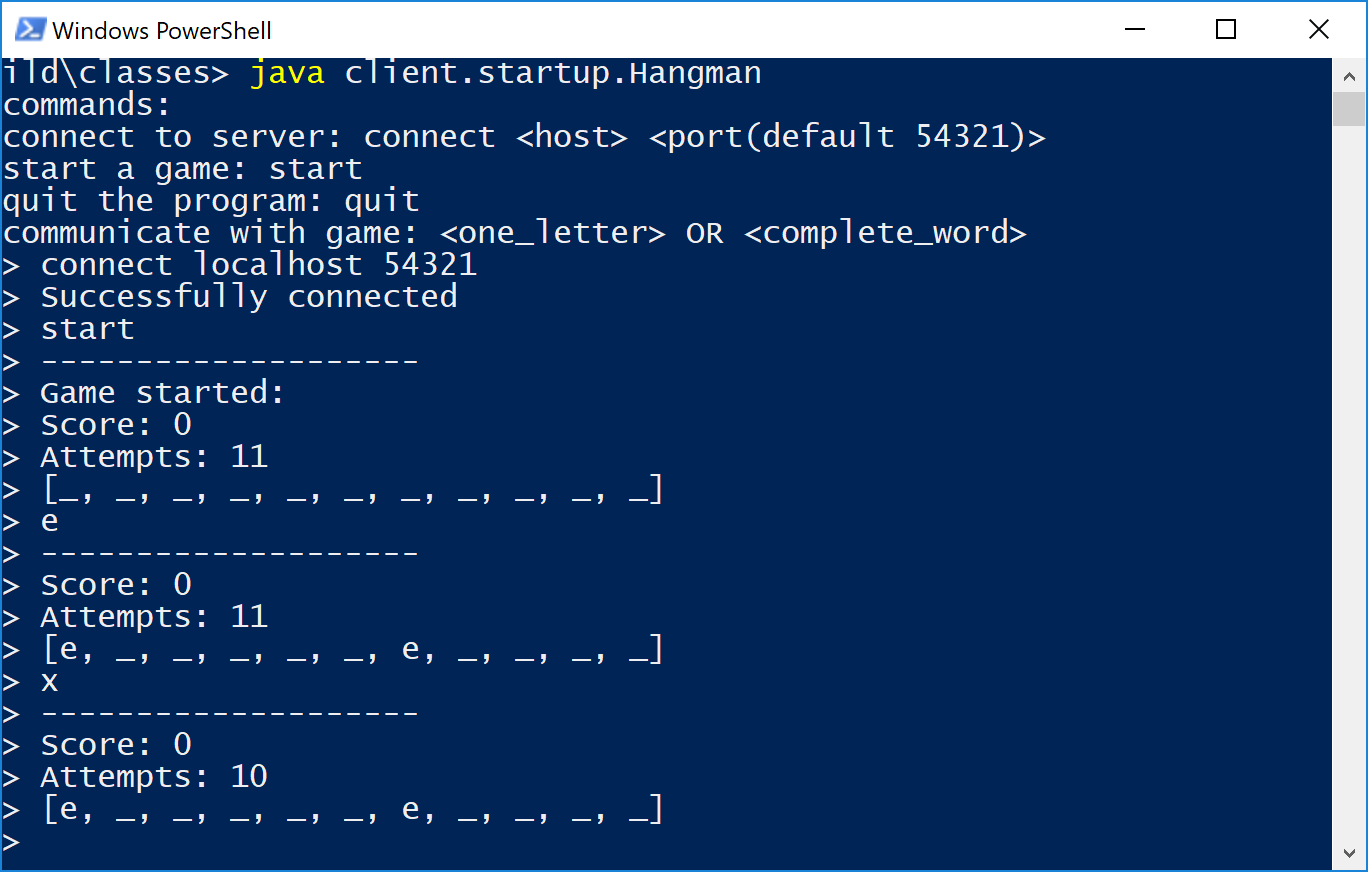
\includegraphics[scale=0.8]{ui.png}
    \caption{}
    \label{fig:ui}
  \end{center}
\end{figure}

Figure \ref{fig:multiple} shows 2 clients playing at once. Moreover, the timeout used can be seen on the server thread in the right bottom command line.

\begin{figure}[h!]
  \begin{center}
    \includegraphics[scale=0.4]{}
    \caption{Concurrent players.}
    \label{fig:multiple}
  \end{center}
\end{figure}

\section{Discussion}

A slight downside to the approach of using locks, i.e. the synchronized keyword in Java, for accessing the message queue which should be sent to the server.
If the sending takes long, e.g. inserting Thread.sleep(10000) on line 143 (ServerConnection.sendToServer()), and the user types more commands which have to be sent then no _prompts_ are printed instantly.
This is the result of the sendMessage() waiting for the lock to release to be able to queue the command/message.
This dosn't affect the responsiveness per se, since the user is still able to input commands which get executed.

This behaviour can be observer on the provided chat example if Thread.sleep(X) is inserted in ServerConnection.sendToServer() on line 201.


\section{Comments About the Course}



\end{document}
